\section{平面图与 Euler 公式}
\label{sec:04-Discrete-Mathematics/03-Graph-Theory/09}

一块单层电路板上有三个模块，每个都要接到电源、地和时钟三条总线上。同一层的铜箔不许交叉——交叉就是短路。九条走线，画得下吗？

这道题的民间版本更老：三座房子各要接通水、电、燃气，管线铺在地面且互不交叉。把房子和设施都当顶点、每条线路当一条边，两个版本问的是同一件事：完全二分图 \(K_{3,3}\) 能不能画在平面上而边不相交。

和七桥一样，反复尝试总是差一条线，而失败一百次也不构成证明——也许只是画法不够巧。要一次性封死所有画法，需要一个跟画法无关的量。

\subsection{面是画出来的，面数却不是}

若图 \(G\) 能画在平面上，使边只在公共端点处相接，就称 \(G\) 是平面图；具体的一幅不交叉画法叫它的平面嵌入。

推理方向容易搞反：画出来有交叉，不能说明图非平面，换个布局交叉可能就没了。\hyperref[sec:04-Discrete-Mathematics/03-Graph-Theory/01]{``图的语言与度数''}提醒过，边上偶然的交叉点不产生顶点。要证明非平面，必须把所有可能的画法一起排除掉，这正是难点所在。

一幅平面嵌入把平面切成若干连通区域，称为面，其中恰有一个是无界的外部面。同一张图可以有看起来很不一样的嵌入，可面的数目一个也不多、一个也不少。

\begin{center}
\begin{tikzpicture}[x=1cm,y=1cm,font=\small]
  \fill[blue!13] (0,0) -- (2.4,0) -- (1.2,0.72) -- cycle;
  \fill[orange!18] (0,0) -- (1.2,2.0) -- (1.2,0.72) -- cycle;
  \fill[green!16] (2.4,0) -- (1.2,2.0) -- (1.2,0.72) -- cycle;
  \draw[thick,black!70] (0,0) -- (2.4,0) -- (1.2,2.0) -- (0,0);
  \draw[thick,black!70] (1.2,0.72) -- (0,0);
  \draw[thick,black!70] (1.2,0.72) -- (2.4,0);
  \draw[thick,black!70] (1.2,0.72) -- (1.2,2.0);
  \foreach \p in {(0,0),(2.4,0),(1.2,2.0),(1.2,0.72)}{\fill \p circle (2.4pt);}
  \node[font=\footnotesize,black!70] at (2.75,1.75) {外部面};
  \node[font=\footnotesize] at (1.2,-0.95) {\(V=4,\ E=6,\ F=4\)};

  \fill[blue!13] (5.2,0) -- (7.6,0) -- (7.6,1.8) -- cycle;
  \fill[orange!18] (5.2,0) -- (7.6,1.8) -- (5.2,1.8) -- cycle;
  \fill[green!16] (5.2,1.8) -- (5.2,0) -- (7.6,0) .. controls (4.6,-1.5) and (3.5,1.2) .. (5.2,1.8);
  \draw[thick,black!70] (5.2,0) -- (7.6,0) -- (7.6,1.8) -- (5.2,1.8) -- cycle;
  \draw[thick,black!70] (5.2,0) -- (7.6,1.8);
  \draw[thick,black!70] (7.6,0) .. controls (4.6,-1.5) and (3.5,1.2) .. (5.2,1.8);
  \foreach \p in {(5.2,0),(7.6,0),(7.6,1.8),(5.2,1.8)}{\fill \p circle (2.4pt);}
  \node[font=\footnotesize,black!70] at (7.1,2.25) {外部面};
  \node[font=\footnotesize] at (6.2,-0.95) {\(V=4,\ E=6,\ F=4\)};
\end{tikzpicture}

\emph{同一张 \(K_4\) 的两种嵌入。左边是三角形套一个中心点，右边是正方形加两条对角线、其中一条绕到外侧走。三块着色区域的形状全变了，可它们连同外部面始终是四个面，\(V-E+F\) 两边都等于 2。这个数不记录你怎么画，只记录这张图画得下。}
\end{center}

\begin{theorem}[Euler 公式]
设连通平面图的任一平面嵌入有 \(V\) 个顶点、\(E\) 条边、\(F\) 个面，则 \(V-E+F=2\)。
\end{theorem}

证明对边数归纳，骨架只有两句。若图是树，则 \(E=V-1\)，没有环就圈不出任何区域，只剩外部一个面，\(F=1\)，代入即得 2。若图不是树，环上任取一条边 \(e\) 删掉：环的另一半仍能绕行，图保持连通；而环上的边一侧朝环内、一侧朝环外，两侧必是两个不同的面，删掉 \(e\) 后它们合并成一个，面数恰好减一。于是 \(V,E-1,F-1\) 满足归纳假设，而 \(V-(E-1)+(F-1)\) 正是 \(V-E+F\)。

两个条件各挡一种失效，值得分开记。``连通''用在删边那一步：正因为 \(e\) 在环上，删了它图不散架，归纳假设才用得上。外部面必须计入 \(F\)：三角形 \(K_3\) 有 \(V=3,E=3\)，面是内部区域加外部区域共两个，\(3-3+2=2\)；漏掉外部面会得到 1，看着像公式错了，其实是账没记全。

若图有 \(c\) 个连通分量，公式变成 \(V-E+F=1+c\)。理由很短：添 \(c-1\) 条不交叉的边把各分量接起来，每条这样的边不切开任何面，所以 \(F\) 不变而 \(E\) 增加 \(c-1\)，套用连通版本再整理即可。

还有一个视角能解释为什么外部面并不特殊。给平面添一个无穷远点，它在拓扑上就是球面，外部面不过是球面上含着无穷远点的那一面。把球转一转，任何一个面都能当外部面。Euler 公式在球面上原样成立。

\subsection{一条计数式压出来的边数上限}

不变量的用处从这里开始。设 \(G\) 是简单平面图且 \(V\ge 3\)。简单图没有自环和平行边，围不出少于三条边的面，所以每个面的边界至少三条边；每条边至多是两个面的公共边界。双面计数给出 \(3F\le 2E\)，代入 Euler 公式消去 \(F\)：

\[
\begin{aligned}
6&=3V-3E+3F\\
&\le 3V-3E+2E=3V-E,
\end{aligned}
\]

也就是

\[
E\le 3V-6.
\]

平面性是对边密度的硬约束：边数至多随顶点数线性增长，稠密图根本没有机会。再配上握手定理就得到一个更细的结构事实——若每个顶点度数都不小于 6，则 \(2E=\sum_{v}\deg(v)\ge 6V\)，即 \(E\ge 3V\)，与上式矛盾。所以任何简单平面图里，必定存在一个度数不超过 5 的顶点。

这句话看着不起眼，却是通向着色的入口。删掉那个度数不超过 5 的顶点，剩下的图仍是平面图，于是可以接着删，得到一个把顶点逐个剥掉的顺序。反向把顶点一个个加回来时，每个顶点最多面对五个已经染好色的邻居，六种颜色里总有一种没被占用。六色定理就这样从一条计数式里掉出来了。把重排做得更精细一些可以证到五色；四色则需要深得多的构形分析，Euler 公式独自到不了那里，但它已经把关键结构——平面图必有局部稀疏处——摆到了台面上。

同一条公式还顺手解决了另一个古老问题。凸多面体可以绷开成平面图，若每个顶点度数同为 \(d\ge 3\)、每个面的边界同为 \(k\ge 3\) 条边，则 \(dV=2E=kF\)，代入 Euler 公式得

\[
\frac{1}{d}+\frac{1}{k}=\frac{1}{2}+\frac{1}{E}>\frac{1}{2}.
\]

满足它的整数对只有五组，依次对应正四面体、立方体、正八面体、正十二面体和正二十面体。正多面体只有五种，这是一个纯粹的计数结论。

\subsection{回到那九条走线}

\(K_5\) 有 \(V=5\)、\(E=10\)，而上界只允许 \(3\cdot 5-6=9\)。矛盾，\(K_5\) 非平面。

\(K_{3,3}\) 逃过了这一关：\(V=6\)、\(E=9\)，而 \(3V-6=12\)。需要用上更多信息。\(K_{3,3}\) 是二分图，不含奇环，特别是不含三角形，所以每个面的边界至少四条边。双面计数改成 \(4F\le 2E\)，即 \(2F\le E\)，代入 Euler 公式得 \(2\le V-E/2\)，整理成

\[
E\le 2V-4.
\]

而 \(9>2\cdot 6-4=8\)。矛盾。九条走线在单层板上铺不下，与画法的巧拙无关。

\begin{center}
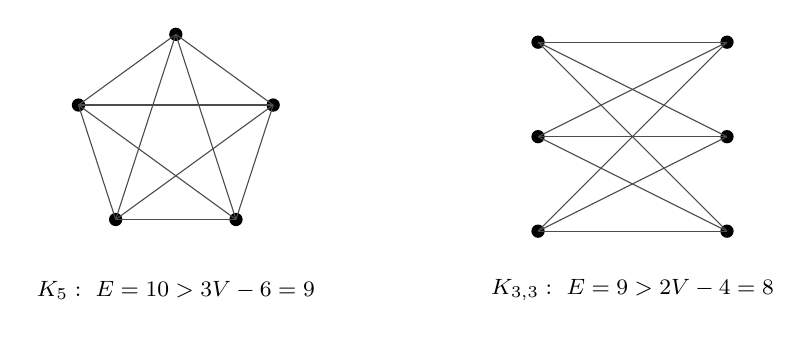
\begin{tikzpicture}[x=1cm,y=1cm,font=\small]
  \foreach \a in {90,162,234,306,18}{\fill (\a:1.3) circle (2.4pt);}
  \foreach \a/\b in {90/162,162/234,234/306,306/18,18/90,90/234,90/306,162/306,162/18,234/18}{
    \draw[black!70] (\a:1.3) -- (\b:1.3);}
  \node[font=\footnotesize] at (0,-1.95) {\(K_5:\ E=10>3V-6=9\)};

  \foreach \y in {1.2,0,-1.2}{\fill (4.6,\y) circle (2.4pt); \fill (7.0,\y) circle (2.4pt);}
  \foreach \y in {1.2,0,-1.2}{\foreach \z in {1.2,0,-1.2}{\draw[black!70] (4.6,\y) -- (7.0,\z);}}
  \node[font=\footnotesize] at (5.8,-1.95) {\(K_{3,3}:\ E=9>2V-4=8\)};
\end{tikzpicture}

\emph{两个基本障碍。左边靠一般的边数上界就否掉了；右边需要先用``二分图没有三角形''把每个面的边界从三条抬到四条，上界才收紧到足以产生矛盾。同一个不变量，喂进去的额外结构不同，挤出来的约束就不同。}
\end{center}

这两个图不是两个孤例。Kuratowski 在 1930 年证明：图非平面，当且仅当它含有 \(K_5\) 或 \(K_{3,3}\) 的细分——把这两张图的边任意替换成串联着若干度数为 2 的中间点的路径所得的图。证明较长，这里只陈述。细分不改变平面性的道理是直观的：在一条边中间插一个度数为 2 的点，只是把一段曲线断成两段；反过来把这些中间点抹平就还原了原来的嵌入。

Wagner 定理是等价的另一种说法，用图 minor（允许删边、删点和收缩边）替代细分。两种语言指向同一对基本图。要留心的是，定理说的是细分或 minor，不是原样出现的子图：一条边被很长的路径替代后，肉眼看不到完全图，障碍却仍然在那里。

顺带说一句对偶。固定一幅连通平面嵌入，把每个面变成顶点，原图每条边分隔的两个面之间连一条边，就得到对偶图 \(G^{*}\)，其中 \(V(G^{*})=F(G)\)、\(E(G^{*})=E(G)\)、\(F(G^{*})=V(G)\)——Euler 公式在对偶下只是把顶点和面对调。更有用的是它把环换成割：原图中围住一片区域的一圈边，在对偶里恰好切断圈内与圈外的面。这条``环即割''的翻译在本单元最后一节还会以另一种形式出现。

\subsection{平面性是可判定的，而且很快}

Euler 不等式能迅速否掉很多图，却给不出肯定结论：满足 \(E\le 3V-6\) 的图未必画得下。Kuratowski 定理给出充要刻画，直接枚举所有细分却不是高效做法。实际的平面性测试有 \(O(\abs{V}+\abs{E})\) 的线性时间算法，而且不只回答是或否——是，就产出一幅嵌入；否，就提取出一个 \(K_5\) 或 \(K_{3,3}\) 的细分当作证书。上一节讨论的证书不对称，在这里恰好两侧都有着落。

结论的适用范围绑在``平面''这两个字上。\(K_5\) 在平面和球面上画不下，在环面上却铺得开。对有 \(g\) 个把手的可定向闭曲面，公式变成

\[
V-E+F=2-2g,
\]

本节所有边数上界都以 \(g=0\) 为前提。电路板做成多层、道路修了立交、管线可以走隧道，物理约束已经改变，平面图的结论不能原样搬。回到开头那块板子：铺不下的是单层，两层就没有问题。

平面图另一副面孔是着色。地图相邻区域不同色，把区域缩成顶点、共享边界的连边，就转成平面图的顶点着色，\hyperref[sec:04-Discrete-Mathematics/03-Graph-Theory/05]{``图着色与冲突安排''}引用过的四颜色定理说四种颜色总够。它的历史很能说明这条路有多陡：1852 年 Guthrie 提出猜想，1879 年 Kempe 的``证明''被接受了十一年才被 Heawood 找出漏洞（Heawood 转而证明了五色定理），1976 年 Appel 与 Haken 把问题归结为一大批不可避免的构形并交给计算机逐一检验，成为数学史上第一个重大的计算机辅助证明，也随即引发争议；2005 年 Gonthier 用证明助手 Coq 给出可机器验证的形式化证明，争议才基本平息。

三屋三井最后交给我们的不只是``铺不下''这个答案。抽象把房屋与设施换成 \(K_{3,3}\)，二分结构把每个面的最短边界从三抬到四，Euler 公式再把``能不能画''压成一条算术矛盾。每一步都扔掉了管线的长短弯曲，又一点没扔掉判断所需的信息。

\(V-E+F\) 之所以有用，正是因为它不随画法变化。下一节把这类量本身当成研究对象：判断两张图是不是同一张图时，不变量是最顺手的工具，也有一个说不上去的天花板。
